\documentclass[aspectratio=169]{beamer}
\usetheme{Madrid}
\usecolortheme{default}

\usepackage{graphicx}
\usepackage{tikz}
\usepackage{amsmath}
\usepackage{algorithm}
\usepackage{algorithmic}
\usepackage{booktabs}
\usetikzlibrary{shapes.geometric, arrows, positioning, fit, backgrounds}

% Define colors
\definecolor{nodecolor1}{RGB}{100,150,200}
\definecolor{nodecolor2}{RGB}{200,100,150}
\definecolor{nodecolor3}{RGB}{150,200,100}
\definecolor{gnnblue}{RGB}{70,130,180}
\definecolor{gnngreen}{RGB}{60,179,113}
\definecolor{gnnorange}{RGB}{255,140,0}

% Title page information
\title[GraphMind: Multi-Agent LLM Topologies]{GraphMind: Efficiently Exploring Multi-Agent LLM Topologies with Graph Neural Networks}
\author{Vito Levstik and Gal Zmazek}
\institute{University of Ljubljana}
\date{\today}

\setbeamertemplate{note page}[plain]
% Uncomment the line below if you want notes on second screen (requires pgfpages)
% \usepackage{pgfpages}
% \setbeameroption{show notes on second screen=right}

\begin{document}

% Title Slide
\begin{frame}
    \titlepage
    \note[item]{Welcome! Today we'll present GraphMind, a framework for efficiently exploring multi-agent LLM topologies}
    \note[item]{This is joint work with Vito Levstik at University of Ljubljana}
    \note[item]{The core idea: use GNNs to predict which agent configurations will work best, avoiding expensive LLM evaluations}
\end{frame}

% Slide 2: The Problem
\begin{frame}{The Challenge: Topology Search is Expensive}
    \begin{columns}[T]
        \begin{column}{0.5\textwidth}
            \textbf{The Problem:}
            \begin{itemize}
                \item Multi-agent LLM systems need configuration
                \item Which agents? How to connect them?
                \item \alert{Combinatorial explosion:} millions of possible graphs
                \item Each evaluation requires many LLM API calls
                \item \textbf{Cost: \$\$\$ + Time}
            \end{itemize}
            
            \vspace{0.5cm}
            \textbf{Our Solution:}
            \\Use GNNs as surrogate models to predict performance
        \end{column}
        \begin{column}{0.5\textwidth}
            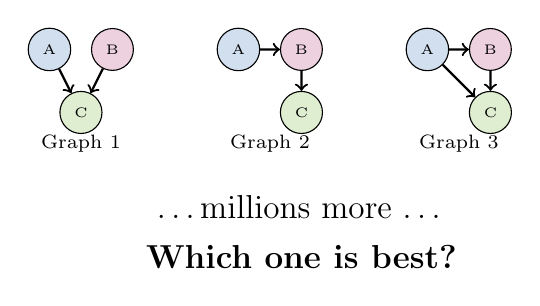
\begin{tikzpicture}[scale=0.8]
                % Draw multiple possible graph topologies
                \node[draw, circle, fill=nodecolor1!30] (a1) at (0,2) {\tiny A};
                \node[draw, circle, fill=nodecolor2!30] (b1) at (1,2) {\tiny B};
                \node[draw, circle, fill=nodecolor3!30] (c1) at (0.5,1) {\tiny C};
                \draw[->, thick] (a1) -- (c1);
                \draw[->, thick] (b1) -- (c1);
                \node at (0.5, 0.5) {\scriptsize Graph 1};
                
                \node[draw, circle, fill=nodecolor1!30] (a2) at (3,2) {\tiny A};
                \node[draw, circle, fill=nodecolor2!30] (b2) at (4,2) {\tiny B};
                \node[draw, circle, fill=nodecolor3!30] (c2) at (4,1) {\tiny C};
                \draw[->, thick] (a2) -- (b2);
                \draw[->, thick] (b2) -- (c2);
                \node at (3.5, 0.5) {\scriptsize Graph 2};
                
                \node[draw, circle, fill=nodecolor1!30] (a3) at (6,2) {\tiny A};
                \node[draw, circle, fill=nodecolor2!30] (b3) at (7,2) {\tiny B};
                \node[draw, circle, fill=nodecolor3!30] (c3) at (7,1) {\tiny C};
                \draw[->, thick] (a3) -- (c3);
                \draw[->, thick] (b3) -- (c3);
                \draw[->, thick] (a3) -- (b3);
                \node at (6.5, 0.5) {\scriptsize Graph 3};
                
                \node at (4, -0.5) {\large \ldots millions more \ldots};
                
                \node at (4, -1.3) {\large \textbf{Which one is best?}};
            \end{tikzpicture}
        \end{column}
    \end{columns}
    
    \note[item]{Start by explaining the core challenge: configuring multi-agent systems is like finding a needle in a haystack}
    \note[item]{With 8 agent types and up to 8 nodes per graph, we have millions of possible configurations}
    \note[item]{Each evaluation requires running LLM API calls - expensive in both time and money}
    \note[item]{Traditional approaches: random search (inefficient), expert design (doesn't scale), exhaustive search (impossible)}
    \note[item]{Our solution: train a GNN to predict which graphs will perform well, then only evaluate the most promising ones}
\end{frame}

% Slide 3: Multi-Agent System Overview
\begin{frame}{Multi-Agent System for Mathematical Problem Solving}
    \begin{columns}[T]
        \begin{column}{0.55\textwidth}
            \textbf{8 Specialized Agent Types:}
            \begin{itemize}
                \item \textcolor{blue}{Solver}: Generate solutions
                \item \textcolor{blue}{Python\_solver}: Execute code
                \item \textcolor{blue}{Validator}: Check correctness
                \item \textcolor{blue}{Extract\_topic}: Identify concepts
                \item \textcolor{blue}{Decompose}: Break into subproblems
                \item \textcolor{blue}{Split}: Parallel exploration
                \item \textcolor{blue}{Combine\_all}: Merge results
                \item \textcolor{blue}{Explain}: Provide reasoning
            \end{itemize}
            
            \vspace{0.3cm}
            \small Task: Solve math problems from NVIDIA OpenMathInstruct-1 dataset
        \end{column}
        \begin{column}{0.45\textwidth}
            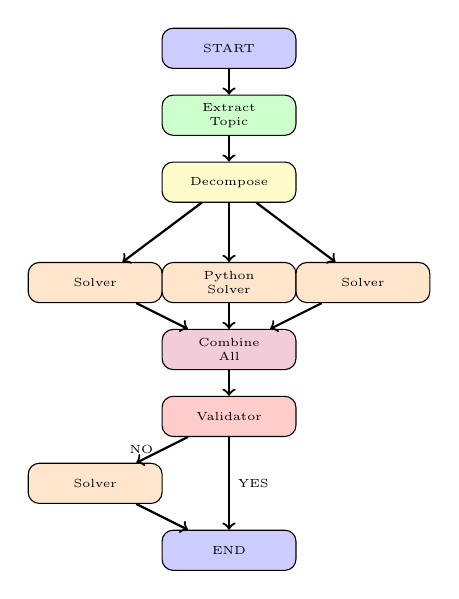
\begin{tikzpicture}[
                node/.style={rectangle, draw, rounded corners, minimum width=2cm, minimum height=0.6cm, align=center, font=\tiny},
                scale=0.85, transform shape
            ]
                \node[node, fill=blue!20] (start) at (0,5) {START};
                \node[node, fill=green!20] (extract) at (0,4) {Extract\\Topic};
                \node[node, fill=yellow!20] (decomp) at (0,3) {Decompose};
                \node[node, fill=orange!20] (solver1) at (-2,1.5) {Solver};
                \node[node, fill=orange!20] (solver2) at (0,1.5) {Python\\Solver};
                \node[node, fill=orange!20] (solver3) at (2,1.5) {Solver};
                \node[node, fill=purple!20] (combine) at (0,0.5) {Combine\\All};
                \node[node, fill=red!20] (valid) at (0,-0.5) {Validator};
                \node[node, fill=orange!20] (solver_retry) at (-2,-1.5) {Solver};
                \node[node, fill=blue!20] (end) at (0,-2.5) {END};
                
                \draw[->, thick] (start) -- (extract);
                \draw[->, thick] (extract) -- (decomp);
                \draw[->, thick] (decomp) -- (solver1);
                \draw[->, thick] (decomp) -- (solver2);
                \draw[->, thick] (decomp) -- (solver3);
                \draw[->, thick] (solver1) -- (combine);
                \draw[->, thick] (solver2) -- (combine);
                \draw[->, thick] (solver3) -- (combine);
                \draw[->, thick] (combine) -- (valid);
                \draw[->, thick] (valid) -- node[right, font=\tiny] {YES} (end);
                \draw[->, thick] (valid) -- node[left, font=\tiny] {NO} (solver_retry);
                \draw[->, thick] (solver_retry) -- (end);
            \end{tikzpicture}
        \end{column}
    \end{columns}
    
    \note[item]{We focus on mathematical problem solving as our test domain}
    \note[item]{8 specialized agent types, each with a specific role in the problem-solving process}
    \note[item]{Agents communicate by passing information along edges in a directed graph}
    \note[item]{Example shown: extract topic, decompose problem, solve in parallel, combine, validate}
    \note[item]{Notice: Validator creates conditional paths - YES goes to END, NO triggers another Solver attempt}
    \note[item]{Different topologies can yield dramatically different performance}
\end{frame}

% Slide 4: Pipeline Overview
\begin{frame}{GraphMind Pipeline: 6-Step Iterative Process}
    \centering
    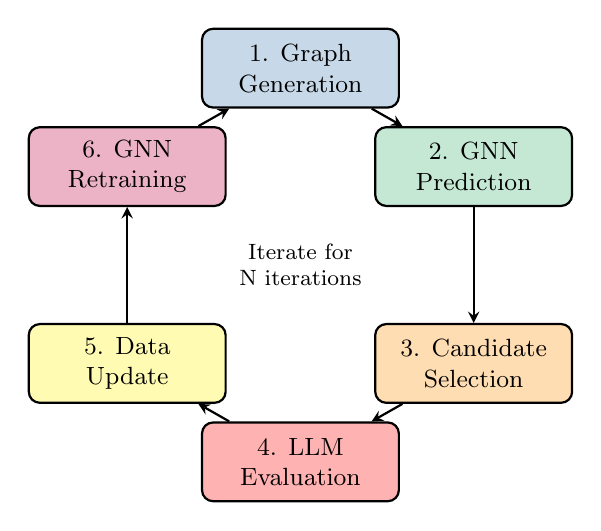
\begin{tikzpicture}[
        box/.style={rectangle, draw, rounded corners, minimum width=2.5cm, minimum height=1cm, align=center, font=\small, thick},
        arrow/.style={->, thick, >=stealth}
    ]
        % Boxes arranged in a regular hexagon
        \node[box, fill=gnnblue!30] (gen) at (4,3.5) {1. Graph\\Generation};
        \node[box, fill=gnngreen!30] (pred) at (6.2,2.25) {2. GNN\\Prediction};
        \node[box, fill=gnnorange!30] (sel) at (6.2,-0.25) {3. Candidate\\Selection};
        \node[box, fill=red!30] (eval) at (4,-1.5) {4. LLM\\Evaluation};
        \node[box, fill=yellow!30] (update) at (1.8,-0.25) {5. Data\\Update};
        \node[box, fill=purple!30] (retrain) at (1.8,2.25) {6. GNN\\Retraining};
        
        % Arrows connecting hexagon vertices
        \draw[arrow] (gen) -- (pred);
        \draw[arrow] (pred) -- (sel);
        \draw[arrow] (sel) -- (eval);
        \draw[arrow] (eval) -- (update);
        \draw[arrow] (update) -- (retrain);
        \draw[arrow] (retrain) -- (gen);
        
        % Central annotation
        \node[font=\footnotesize, align=center] at (4, 1) {Iterate for\\N iterations};
    \end{tikzpicture}
    
    \vspace{0.5cm}
    \textbf{Key Idea:} Generate many candidates → GNN filters → Evaluate only the best → Improve GNN
    
    \note[item]{This is our core pipeline - an iterative 6-step process}
    \note[item]{Step 1: Generate 200k random candidate graphs}
    \note[item]{Step 2: GNN predicts performance for all candidates}
    \note[item]{Step 3: Select top 10 based on predictions, evaluate top 5}
    \note[item]{Step 4: Actually run those graphs with LLMs on math problems}
    \note[item]{Step 5: Add results to training data}
    \note[item]{Step 6: Retrain GNN on expanded dataset}
    \note[item]{Each iteration improves the GNN's ability to identify good graphs}
\end{frame}

% Slide 5: Step 1 - Graph Generation
\begin{frame}{Step 1: Graph Generation}
    \begin{columns}[T]
        \begin{column}{0.5\textwidth}
            \textbf{Semi-Random Generation:}
            \begin{itemize}
                \item Generate 200,000 graphs per iteration
                \item Constraints: max 8 nodes, max depth 3
                \item Rules enforce structure:
                \begin{itemize}
                    \item Decompose\_3 → 3 branches
                    \item Combine\_all merges branches
                    \item START and END nodes
                \end{itemize}
                \item Filter duplicates
                \item Result: 1,000-2,000 unique graphs
            \end{itemize}
        \end{column}
        \begin{column}{0.5\textwidth}
            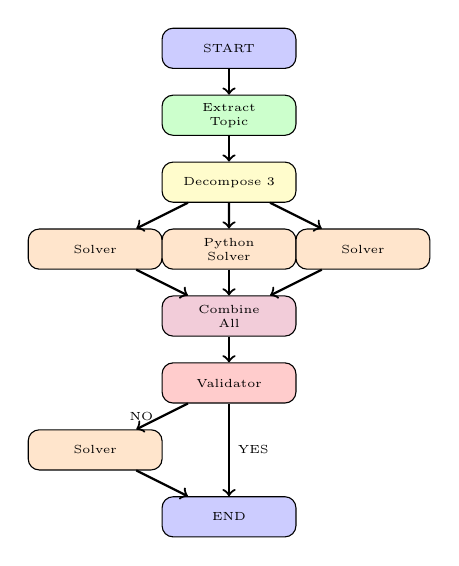
\begin{tikzpicture}[
                node/.style={rectangle, draw, rounded corners, minimum width=2cm, minimum height=0.6cm, align=center, font=\tiny},
                scale=0.85, transform shape
            ]
                \node[node, fill=blue!20] (start) at (0,4.5) {START};
                \node[node, fill=green!20] (extract) at (0,3.5) {Extract\\Topic};
                \node[node, fill=yellow!20] (decomp) at (0,2.5) {Decompose 3};
                \node[node, fill=orange!20] (solver1) at (-2,1.5) {Solver};
                \node[node, fill=orange!20] (solver2) at (0,1.5) {Python\\Solver};
                \node[node, fill=orange!20] (solver3) at (2,1.5) {Solver};
                \node[node, fill=purple!20] (combine) at (0,0.5) {Combine\\All};
                \node[node, fill=red!20] (valid) at (0,-0.5) {Validator};
                \node[node, fill=orange!20] (solver_retry) at (-2,-1.5) {Solver};
                \node[node, fill=blue!20] (end) at (0,-2.5) {END};
                
                \draw[->, thick] (start) -- (extract);
                \draw[->, thick] (extract) -- (decomp);
                \draw[->, thick] (decomp) -- (solver1);
                \draw[->, thick] (decomp) -- (solver2);
                \draw[->, thick] (decomp) -- (solver3);
                \draw[->, thick] (solver1) -- (combine);
                \draw[->, thick] (solver2) -- (combine);
                \draw[->, thick] (solver3) -- (combine);
                \draw[->, thick] (combine) -- (valid);
                \draw[->, thick] (valid) -- node[right, font=\tiny] {YES} (end);
                \draw[->, thick] (valid) -- node[left, font=\tiny] {NO} (solver_retry);
                \draw[->, thick] (solver_retry) -- (end);
            \end{tikzpicture}
        \end{column}
    \end{columns}
    
    \note[item]{Step 1 in detail: graph generation}
    \note[item]{Generate 200,000 candidates per iteration using semi-random recursive algorithm}
    \note[item]{Not completely random - follow structural rules like Decompose must split into branches}
    \note[item]{Constraints: max 8 nodes, max depth 3 to keep graphs manageable}
    \note[item]{Filter duplicates - end up with 1000-2000 unique graphs}
    \note[item]{Example shown: Decompose splits into 3 solvers, Combine merges results, Validator checks with conditional paths}
    \note[item]{Validator creates branching: if validation passes (YES) go to END, if fails (NO) retry with another Solver}
\end{frame}

% Slide 6: Step 2 - GNN Prediction
\begin{frame}{Step 2: GNN Prediction with Virtual Node}
    \begin{columns}[T]
        \begin{column}{0.5\textwidth}
            \textbf{GNN Architecture:}
            \begin{itemize}
                \item \textbf{Input:} One-hot node features (15 types)
                \item \textbf{Models:} GCN, GraphSAGE, GAT
                \item \textbf{Virtual Node:} Connected to all nodes
                \item \textbf{Message Passing:} 2-4 layers
                \item \textbf{Output:} Score $\in$ [0,1] via sigmoid
            \end{itemize}
            
            \vspace{0.3cm}
            \textbf{Virtual Node Technique:}
            \begin{itemize}
                \item Aggregates global graph information
                \item Final embedding → MLP → prediction
                \item Enables graph-level predictions
            \end{itemize}
        \end{column}
        \begin{column}{0.5\textwidth}
            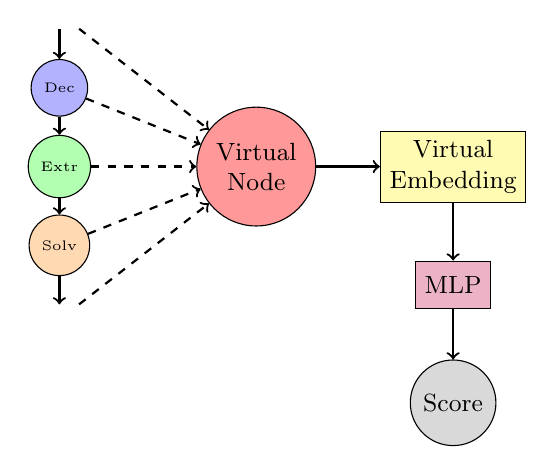
\begin{tikzpicture}[scale=0.5]
                % Graph nodes (even smaller, left side)
                \node[draw, circle, fill=blue!30, font=\tiny, minimum size=0.5cm] (n1) at (0,4) {Dec};
                \node[draw, circle, fill=green!30, font=\tiny, minimum size=0.5cm] (n2) at (0,2) {Extr};
                \node[draw, circle, fill=orange!30, font=\tiny, minimum size=0.5cm] (n3) at (0,0) {Solv};
                
                % Graph edges
                \draw[->, thick] (0,5.5) -- (n1);
                \draw[->, thick] (n1) -- (n2);
                \draw[->, thick] (n2) -- (n3);
                \draw[->, thick] (n3) -- (0,-1.5);

                % Virtual node
                \node[draw, circle, fill=red!40, font=\small, minimum size=0.8cm, align=center] (vnode) at (5,2) {Virtual\\Node};

                % Connections to virtual node
                \draw[->, dashed, thick] (n1) -- (vnode);
                \draw[->, dashed, thick] (n2) -- (vnode);
                \draw[->, dashed, thick] (n3) -- (vnode);
                \draw[->, dashed, thick] (0.5,5.5) -- (vnode);
                \draw[->, dashed, thick] (0.5,-1.5) -- (vnode);

                % Embedding to MLP
                \node[draw, rectangle, fill=yellow!30, font=\small, minimum size=0.6cm, align=center] (vemb) at (10,2) {Virtual\\Embedding};
                \draw[->, thick] (vnode) -- (vemb);
                \node[draw, rectangle, fill=purple!30, font=\small, minimum size=0.6cm] (mlp) at (10,-1) {MLP};
                \draw[->, thick] (vemb) -- (mlp);

                % Output score
                \node[draw, circle, fill=gray!30, font=\small, minimum size=0.6cm] (out) at (10,-4) {Score};
                \draw[->, thick] (mlp) -- (out);
                
                
            \end{tikzpicture}
        \end{column}
    \end{columns}
    
    \note[item]{Step 2: GNN makes predictions for all 1000-2000 candidates}
    \note[item]{Input: one-hot encoded node types - 15 dimensional vectors}
    \note[item]{Tested three GNN architectures: GCN, GraphSAGE, and GAT}
    \note[item]{Key innovation: virtual node technique for graph-level prediction}
    \note[item]{Virtual node is connected to all other nodes, aggregates global information}
    \note[item]{After message passing, virtual node embedding goes through MLP and sigmoid}
    \note[item]{Output: predicted accuracy score between 0 and 1}
    \note[item]{In first iteration, no training data exists, so we make random predictions}
\end{frame}

% Slide 7: Steps 3-4 - Selection and Evaluation
\begin{frame}{Steps 3-4: Selection and LLM Evaluation}
    \begin{columns}[T]
        \begin{column}{0.5\textwidth}
            \textbf{Step 3: Candidate Selection}
            \begin{itemize}
                \item Top 10 graphs → candidate pool
                \item Select top 5 for evaluation
                \item Pool size limited to 10
                \item Removes lowest-scoring graphs
            \end{itemize}
            
            \vspace{0.5cm}
            \textbf{Step 4: LLM Evaluation}
            \begin{itemize}
                \item Build LangGraph from structure
                \item Evaluate on 5 math problems
                \item Each agent makes LLM calls
                \item \alert{Thousands of API calls!}
                \item Score: exact match or relative error
            \end{itemize}
        \end{column}
        \begin{column}{0.5\textwidth}
            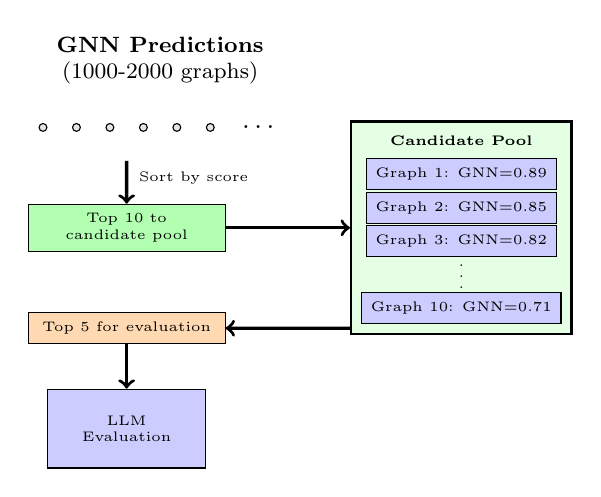
\begin{tikzpicture}[scale=0.85]
                % Selection visualization
                \node[font=\footnotesize, align=center] at (0, 5) {\textbf{GNN Predictions}\\(1000-2000 graphs)};
                
                \foreach \i in {1,...,6} {
                    \node[draw, circle, fill=gray!20, inner sep=1pt, font=\tiny] at ({(\i-4.5)*0.5}, 4) {};
                }
                \node at (1.5, 4) {\ldots};
                
                
                \node[font=\tiny] at (0.5, 3.25) {Sort by score};
                
                % Top candidates - arrow pointing to candidate pool
                \node[draw, rectangle, fill=green!30, minimum width=2.5cm, font=\tiny, align=center] (top10) at (-0.5, 2.5) {Top 10 to\\candidate pool};
                \draw[->, very thick] (-0.5, 3.5) -- (top10.north);

                % Candidate Pool visualization (further to the right)
                \node[draw, rectangle, fill=green!10, minimum width=2.8cm, minimum height=2.7cm, font=\tiny, thick] (pool) at (4.5, 2.5) {};
                \node[font=\tiny, align=center] at (4.5, 3.8) {\textbf{Candidate Pool}};
                
                % Graphs in pool with GNN scores
                \node[draw, rectangle, fill=blue!20, font=\tiny, minimum width=2.4cm] at (4.5, 3.3) {Graph 1: GNN=0.89};
                \node[draw, rectangle, fill=blue!20, font=\tiny, minimum width=2.4cm] at (4.5, 2.8) {Graph 2: GNN=0.85};
                \node[draw, rectangle, fill=blue!20, font=\tiny, minimum width=2.4cm] at (4.5, 2.3) {Graph 3: GNN=0.82};
                \node[font=\tiny] at (4.5, 1.9) {\vdots};
                \node[draw, rectangle, fill=blue!20, font=\tiny, minimum width=2.4cm] at (4.5, 1.3) {Graph 10: GNN=0.71};
                
                % Arrow from top10 to pool
                \draw[->, very thick] (top10.east) -- (pool.west);

                % Selected for evaluation
                \node[draw, rectangle, fill=orange!30, minimum width=2.5cm, font=\tiny] (top5eval) at (-0.5, 1) {Top 5 for evaluation};
                
                \draw[->, very thick] (2.85, 1) -- (top5eval.east);
                
                % LLM evaluation
                \node[draw, rectangle, fill=blue!20, minimum width=2cm, minimum height=1cm, font=\tiny, align=center] (llm) at (-0.5, -0.5) {LLM\\Evaluation};

                \draw[->, very thick] (top5eval.south) -- (llm.north);

            \end{tikzpicture}
        \end{column}
    \end{columns}
    
    \note[item]{Step 3: From 1000-2000 candidates, select the most promising ones}
    \note[item]{Top 10 go into candidate pool, stored with their GNN predicted scores}
    \note[item]{Candidate pool shown on right: graphs ranked by GNN score (0.89, 0.85, etc.)}
    \note[item]{Pool maintains best graphs across iterations, limited to size 10}
    \note[item]{Step 4: The expensive part - actual LLM evaluation}
    \note[item]{Build executable LangGraph from graph structure using agent functions}
    \note[item]{Run on 5 math problems from NVIDIA OpenMathInstruct-1 dataset}
    \note[item]{Each agent in the graph may make multiple LLM API calls}
    \note[item]{This generates thousands of LLM requests per iteration - expensive!}
    \note[item]{Scoring: exact match gets 1.0, numerical answers use relative error}
\end{frame}

% Slide 8: Steps 5-6 - Update and Retrain
\begin{frame}{Steps 5-6: Data Update and GNN Retraining}
    \begin{columns}[T]
        \begin{column}{0.5\textwidth}
            \textbf{Step 5: Data Update}
            \begin{itemize}
                \item Add evaluated graphs to training set
                \item Each graph: structure + true score
                \item Dataset grows by 5 graphs/iteration
                \item Accumulates over iterations
            \end{itemize}
            
            \vspace{0.5cm}
            \textbf{Step 6: GNN Retraining}
            \begin{itemize}
                \item Retrain every iteration
                \item Supervised learning: MSE loss
                \item Adam optimizer
                \item 300 epochs, batch size 32
                \item Model learns structure-performance mapping
            \end{itemize}
        \end{column}
        \begin{column}{0.5\textwidth}
            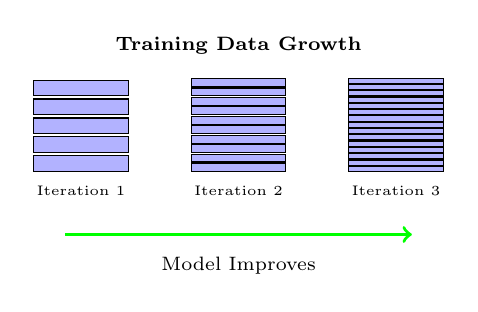
\begin{tikzpicture}[scale=0.8]
                % Training data growth
                \foreach \i in {0,...,4} {
                    \draw[fill=blue!30] (0, \i*0.3) rectangle (1.5, \i*0.3+0.25);
                }
                \node[font=\tiny] at (0.75, -0.3) {Iteration 1};
                
                \foreach \i in {0,...,9} {
                    \draw[fill=blue!30] (2.5, \i*0.15) rectangle (4, \i*0.15+0.125);
                }
                \node[font=\tiny] at (3.25, -0.3) {Iteration 2};
                
                \foreach \i in {0,...,14} {
                    \draw[fill=blue!30] (5, \i*0.1) rectangle (6.5, \i*0.1+0.083);
                }
                \node[font=\tiny] at (5.75, -0.3) {Iteration 3};
                
                \node[font=\scriptsize, align=center] at (3.25, 2) {\textbf{Training Data Growth}};
                
                % Improvement arrow
                \draw[->, very thick, green] (0.5, -1) -- (6, -1);
                \node[font=\scriptsize] at (3.25, -1.5) {Model Improves};
                
            \end{tikzpicture}
        \end{column}
    \end{columns}
    
    \vspace{0.3cm}
    \textbf{Result:} GNN becomes better at predicting performance from structure
    
    \note[item]{Step 5: Add the 5 evaluated graphs to our training dataset}
    \note[item]{Each graph is a training example: structure plus its true accuracy score}
    \note[item]{Dataset starts small, grows by 5 graphs each iteration}
    \note[item]{Step 6: Retrain the GNN on expanded dataset}
    \note[item]{Standard supervised learning with MSE loss}
    \note[item]{Train for 300 epochs with Adam optimizer}
    \note[item]{GNN learns to map graph structure to performance}
    \note[item]{With each iteration, model gets better at identifying promising graphs}
    \note[item]{This completes one iteration - cycle repeats for 30 iterations total}
\end{frame}

% Slide 9: Random Baseline Distribution
\begin{frame}{Random Baseline: Understanding the Distribution}
    \begin{columns}[T]
        \begin{column}{0.55\textwidth}
            \textbf{Establishing a Baseline:}
            \begin{itemize}
                \item Generated 5M random graphs
                \item Sampled 150 for evaluation
                \item Measured performance on math problems
                \item Analyzed score distribution
            \end{itemize}
            
            \textbf{Observed: Bimodal Distribution}
            \begin{itemize}
                \item Two clusters: good ($>0.5$) and poor ($<0.3$)
                \item Simple distributions insufficient
            \end{itemize}

            \textbf{Solution: Gaussian Mixture Model}
            \begin{itemize}
                \item GMM with 2 components
                \item Fitted using EM algorithm
                \item Captures bimodal structure
                \item Baseline for comparison
            \end{itemize}
        \end{column}
        \begin{column}{0.45\textwidth}
            \centering
            
\includegraphics[width=\textwidth]{score_distribution.png}
            
            \vspace{0.3cm}
            \small
            Random graph distribution fitted with GMM\\
            \textbf{Two clusters:} good and poor performing graphs
        \end{column}
    \end{columns}
    
    \note[item]{Before evaluating our GNN approach, we established a random baseline}
    \note[item]{Generated 5 million random graphs, sampled 150 for evaluation}
    \note[item]{Observed bimodal distribution - two distinct clusters of performance}
    \note[item]{Good graphs score above 0.5, poor graphs below 0.3}
    \note[item]{Simple parametric distributions like Beta or Normal couldn't capture this}
    \note[item]{Used Gaussian Mixture Model with 2 components - fitted using EM algorithm}
    \note[item]{GMM captures the bimodal structure and provides our baseline for comparison}
    \note[item]{This shows what we'd get from pure random search}
\end{frame}

% Slide 10: GNN Models and Hyperparameters
\begin{frame}{GNN Models: Architecture Details}
    \begin{columns}[T]
        \begin{column}{0.6\textwidth}
            \textbf{Three GNN Architectures:}
            \begin{enumerate}
                \item \textbf{GCN} (Graph Convolutional Network)
                
                \item \textbf{GraphSAGE}
                
                \item \textbf{GAT} (Graph Attention Network)
            \end{enumerate}
            
            \vspace{0.3cm}
            \textbf{Hyperparameter Search:}
            \begin{itemize}
                \item Layers: [2, 3, 4]
                \item Hidden dim: [4, 8, 16, 32]
                \item Dropout: [0.0, 0.1, 0.2, 0.5]
            \end{itemize}
        \end{column}
        \begin{column}{0.4\textwidth}
            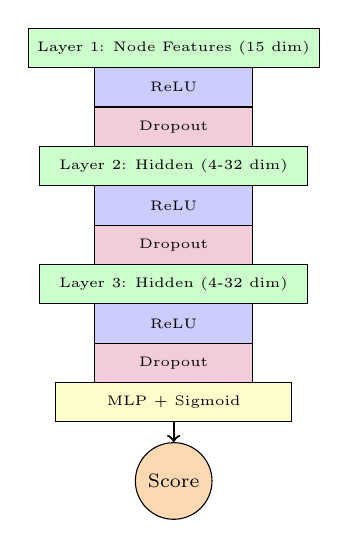
\begin{tikzpicture}[scale=1.0]
                % Layer 1
                \node[draw, rectangle, fill=green!20, minimum width=3.4cm, minimum height=0.5cm, font=\tiny] (l1) at (0, 4) {Layer 1: Node Features (15 dim)};
                \node[draw, rectangle, fill=blue!20, minimum width=2cm, minimum height=0.5cm, font=\tiny] (r1) at (0, 3.5) {ReLU};
                \node[draw, rectangle, fill=purple!20, minimum width=2cm, minimum height=0.5cm, font=\tiny] (d1) at (0, 3) {Dropout};
                % Layer 2
                \node[draw, rectangle, fill=green!20, minimum width=3.4cm, minimum height=0.5cm, font=\tiny] (l2) at (0, 2.5) {Layer 2: Hidden (4-32 dim)};
                \node[draw, rectangle, fill=blue!20, minimum width=2cm, minimum height=0.5cm, font=\tiny] (r2) at (0, 2) {ReLU};
                \node[draw, rectangle, fill=purple!20, minimum width=2cm, minimum height=0.5cm, font=\tiny] (d2) at (0, 1.5) {Dropout};
                % Layer 3
                \node[draw, rectangle, fill=green!20, minimum width=3.4cm, minimum height=0.5cm, font=\tiny] (l3) at (0, 1) {Layer 3: Hidden (4-32 dim)};
                \node[draw, rectangle, fill=blue!20, minimum width=2cm, minimum height=0.5cm, font=\tiny] (r3) at (0, 0.5) {ReLU};
                \node[draw, rectangle, fill=purple!20, minimum width=2cm, minimum height=0.5cm, font=\tiny] (d3) at (0, 0) {Dropout};
                % MLP
                \node[draw, rectangle, fill=yellow!20, minimum width=3cm, minimum height=0.5cm, font=\tiny] (mlp) at (0, -0.5) {MLP + Sigmoid};
                
                % Output
                \node[draw, circle, fill=orange!30, font=\scriptsize] (out) at (0, -1.5) {Score};

                % Arrow
                \draw[->, thick] (mlp.south) -- (out.north);

            \end{tikzpicture}
        \end{column}
    \end{columns}
    
    \note[item]{We tested three GNN architectures}
    \note[item]{GCN: simple and fast, uses spectral graph convolutions}
    \note[item]{GraphSAGE: samples and aggregates from neighborhoods, good for inductive learning}
    \note[item]{GAT: uses attention mechanisms to weight neighbor contributions}
    \note[item]{Performed extensive hyperparameter search on synthetic data first}
    \note[item]{Varied number of layers, hidden dimensions, and dropout rates}
    \note[item]{Architecture shown: typical 4-layer setup with virtual node readout}
    \note[item]{Each layer aggregates information from neighbors}
    \note[item]{Final virtual node embedding contains global graph information}
\end{frame}

% Slide 11: Results - GNN Performance
\begin{frame}{Results: GNN Model Performance}
    \begin{columns}[T]
        \begin{column}{0.5\textwidth}
            \textbf{Hyperparameter Search Results:}
            
            \vspace{0.3cm}
            \small
            \begin{tabular}{lccc}
                \toprule
                \textbf{Model} & \textbf{Layers} & \textbf{Hidden} & \textbf{MSE} \\
                \midrule
                GCN & 4 & 8 & 0.0123 \\
                GraphSAGE & 4 & 16 & 0.0089 \\
                GAT & 4 & 8 & 0.0156 \\
                \bottomrule
            \end{tabular}
            
            \vspace{0.5cm}
            \textbf{Test Performance (10 runs):}
            
            \vspace{0.3cm}
            \small
            \begin{tabular}{lc}
                \toprule
                \textbf{Model} & \textbf{Test MSE} \\
                \midrule
                GCN & 0.0145 ± 0.0021 \\
                GraphSAGE & \textbf{0.0102 ± 0.0018} \\
                GAT & 0.0178 ± 0.0025 \\
                \bottomrule
            \end{tabular}
            
            \vspace{0.3cm}
            \alert{GraphSAGE performs best!}
        \end{column}
        \begin{column}{0.5\textwidth}
            \centering
            \textbf{Key Insights:}
            \begin{itemize}
                \item 4 layers optimal
                \item Hidden dim 8-16 works well
                \item GraphSAGE generalizes best
                \item Low variance across runs
            \end{itemize}
        \end{column}
    \end{columns}
    
    \note[item]{First, we optimized GNN hyperparameters on synthetic data}
    \note[item]{Tested 600 synthetic graphs: 400 training, 200 test}
    \note[item]{10-fold cross-validation for hyperparameter selection}
    \note[item]{Best configurations: 4 layers, hidden dims 8-16, various dropout}
    \note[item]{GraphSAGE achieved lowest test MSE: 0.0102}
    \note[item]{Repeated 10 times to account for randomness - low variance}
    \note[item]{These optimized configurations were used in the main pipeline}
\end{frame}

% Slide 12: The Prediction Paradox - Part 1
\begin{frame}{Pipeline Dynamics: The Prediction Paradox (1/2)}
    \begin{columns}[T]
        \begin{column}{0.5\textwidth}
            \textbf{An Interesting Phenomenon:}
            \begin{itemize}
                \item GNN predictions become very accurate
                \item But... this creates a bias!
                \item Model overfits to its own selections
                \item Training data becomes skewed
            \end{itemize}
            
            \vspace{0.5cm}
            \textbf{The Feedback Loop:}
            \begin{enumerate}
                \item GNN predicts good graphs
                \item \alert{Only predicted "good" graphs evaluated}
                \item Training data biased toward these
                \item GNN learns to predict "more of same"
                \item Diversity decreases over iterations
            \end{enumerate}
        \end{column}
        \begin{column}{0.5\textwidth}
            \centering
            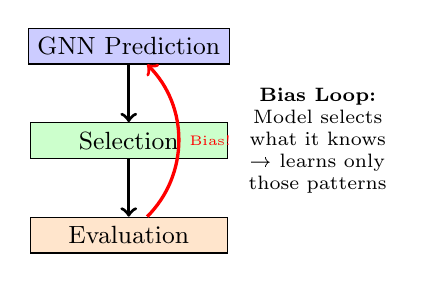
\begin{tikzpicture}[scale=0.8]
                % Feedback loop visualization
                \node[draw, rectangle, fill=blue!20, minimum width=2.5cm, font=\small] (gnn) at (0, 3) {GNN Prediction};
                \node[draw, rectangle, fill=green!20, minimum width=2.5cm, font=\small] (sel) at (0, 1.5) {Selection};
                \node[draw, rectangle, fill=orange!20, minimum width=2.5cm, font=\small] (eval) at (0, 0) {Evaluation};
                
                \draw[->, very thick] (gnn) -- (sel);
                \draw[->, very thick] (sel) -- (eval);
                \draw[->, very thick, red] (eval) to[bend right=45] node[right, font=\tiny] {Bias!} (gnn);
                
                \node[font=\scriptsize, align=center] at (3, 1.5) {\textbf{Bias Loop:}\\Model selects\\what it knows\\→ learns only\\those patterns};
            \end{tikzpicture}
            
            \vspace{0.5cm}
            \small
            \textbf{Result:} Training data becomes increasingly\\
            biased toward model's preferred patterns
        \end{column}
    \end{columns}
    
    \note[item]{An interesting paradox emerged: GNN predictions became very accurate, but this created bias}
    \note[item]{The feedback loop: GNN selects graphs it predicts are good, only those get evaluated}
    \note[item]{Training data becomes increasingly biased toward the types of graphs GNN likes}
    \note[item]{Model learns to predict "more of the same" rather than truly good graphs in general}
    \note[item]{This creates a selection bias that accumulates over iterations}
\end{frame}

% Slide 13: The Prediction Paradox - Part 2
\begin{frame}{Pipeline Dynamics: The Prediction Paradox (2/2)}
    \begin{columns}[T]
        \begin{column}{0.5\textwidth}
            \textbf{Observable in Metrics:}
            \begin{itemize}
                \item RMSE appears to improve
                \item But on biased sample!
                \item GNN score variance increases
                \item Actual diversity decreases
            \end{itemize}
            
            \vspace{0.5cm}
            \textbf{Key Insight:}
            \begin{itemize}
                \item Model becomes "too good" at its own strategy
                \item Reduces exploration of search space
                \item Selection bias accumulates
            \end{itemize}
        \end{column}
        \begin{column}{0.5\textwidth}
            \centering
            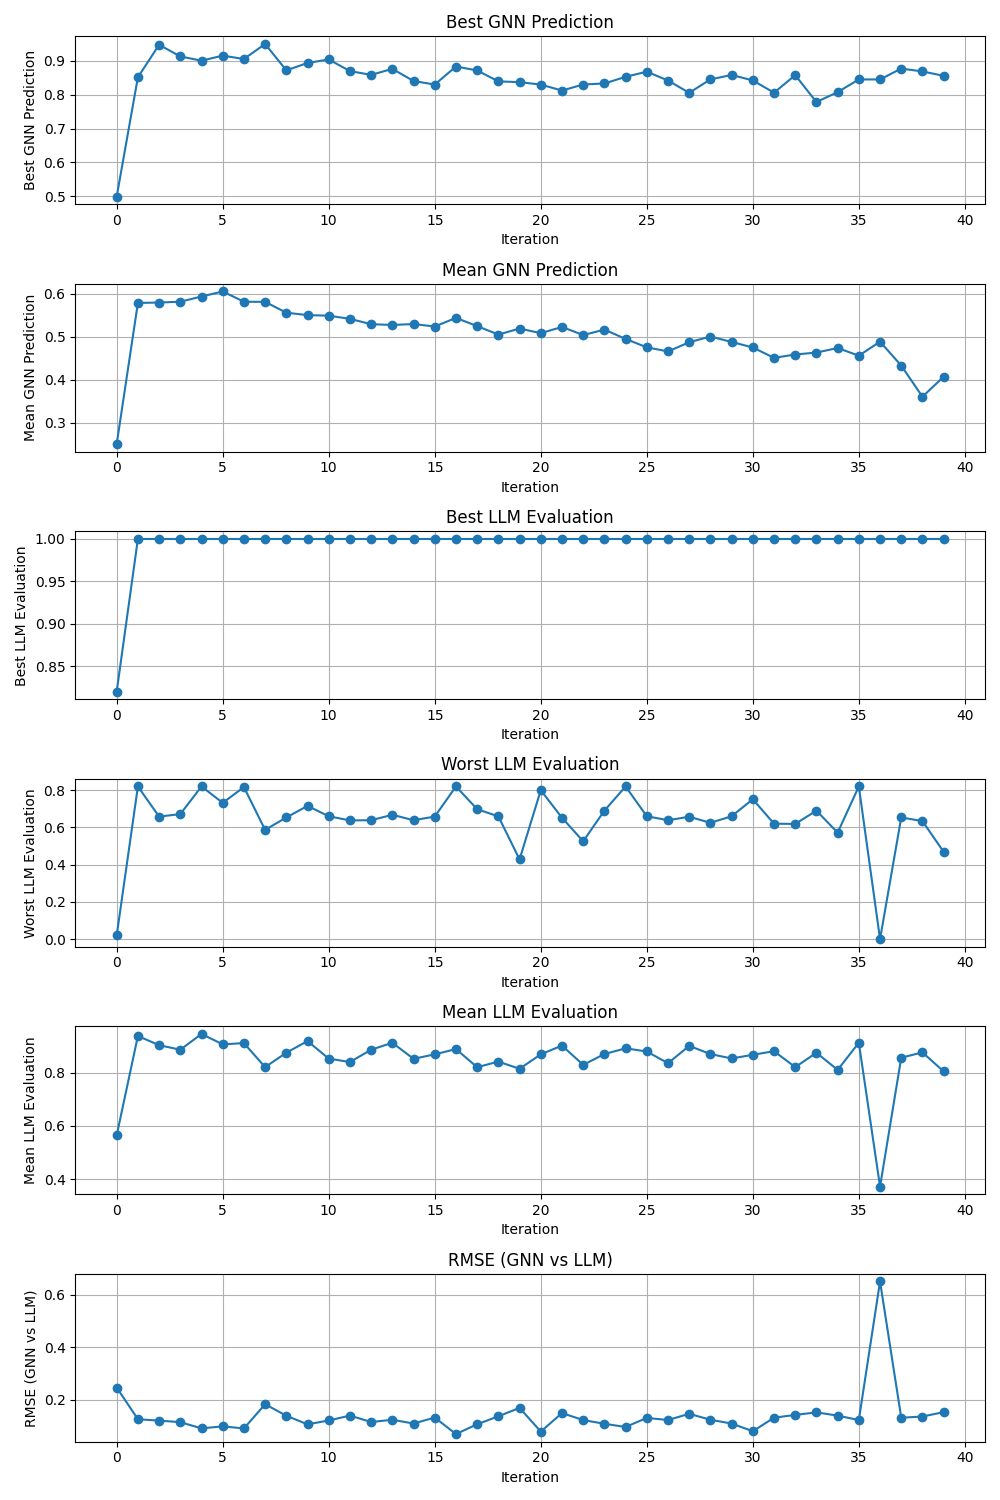
\includegraphics[width=0.6\textwidth]{../logs/analytics/more-agents-real-llm-v4-bestGCN/metric_trends.png}
            
            \vspace{0.3cm}
            \small
            \textbf{Metric trends over 30 iterations}
            
            \vspace{0.2cm}
            Model becomes "too good" at predicting\\
            its own selections, reducing exploration
            
            \vspace{0.3cm}
            \textbf{Future Work:} Stratified sampling to\\
            maintain diversity and avoid bias
        \end{column}
    \end{columns}
    
    \note[item]{This is visible in the metrics: RMSE improves but on increasingly biased sample}
    \note[item]{The model becomes "too good" at its own selection strategy}
    \note[item]{Despite this limitation, approach still significantly outperforms random search}
    \note[item]{Future work: stratified sampling to maintain diversity and avoid this bias}
    \note[item]{This is an honest acknowledgment of limitations while emphasizing success}
\end{frame}

% Slide 14: Results - Distribution Comparison
\begin{frame}{Results: GNN-Guided vs Random Search}
    \begin{columns}[T]
        \begin{column}{0.5\textwidth}
            \textbf{Experimental Setup:}
            \begin{itemize}
                \item \textbf{Baseline:} 150 random graphs
                \item \textbf{GraphMind:} 30 iterations
                \item Each graph evaluated on 10 problems
                \item Modeled random baseline as GMM
            \end{itemize}
            
            \vspace{0.5cm}
            \textbf{Key Results:}
            \begin{itemize}
                \item \alert{GraphSAGE:} Best average (0.72 vs 0.43)
                \item \alert{GAT:} 10\% of graphs scored 1.0
                \item \alert{GCN:} Strong performance (0.69 avg)
                \item All models significantly beat random
            \end{itemize}
        \end{column}
        \begin{column}{0.5\textwidth}
            \centering
            \textbf{Score Distributions}
            
            \vspace{0.2cm}
            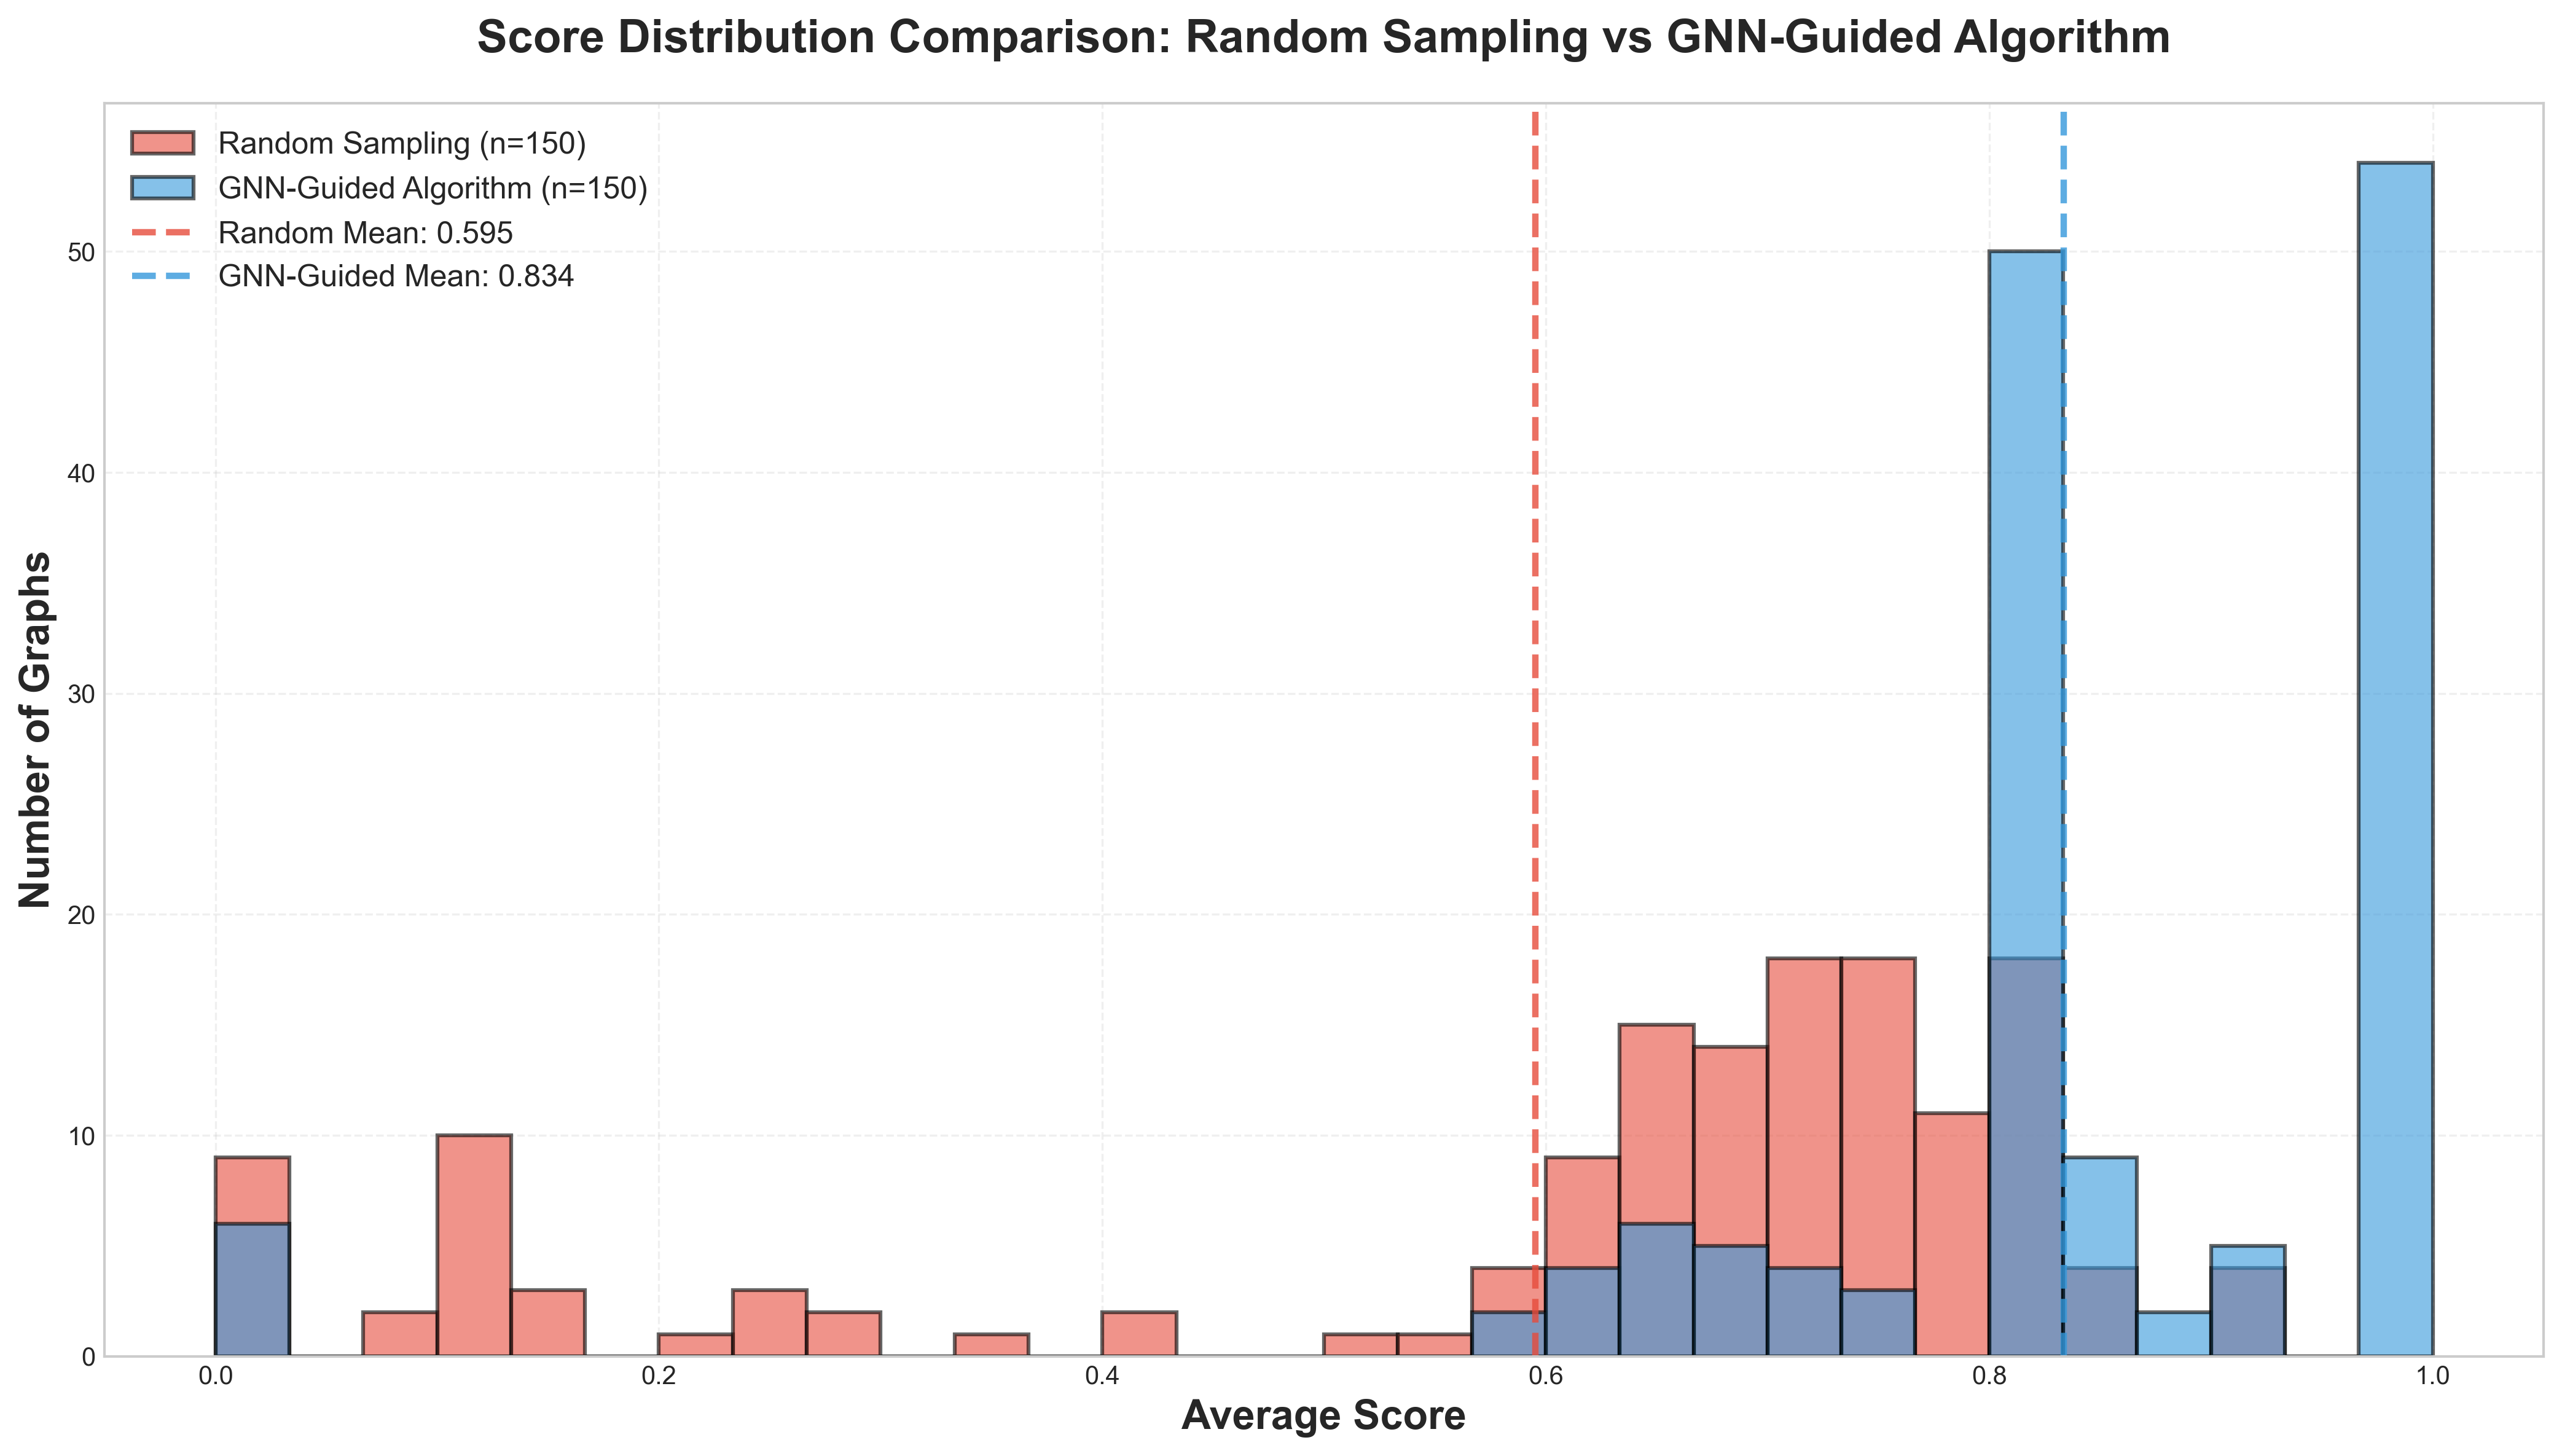
\includegraphics[width=0.95\textwidth]{../reports/blog_images/random_vs_gnn_comparison.png}
            
            \vspace{0.3cm}
            \small
            Random baseline (red) vs GNN-guided search (blue)
        \end{column}
    \end{columns}
    
    \note[item]{Main results: comparing GNN-guided search to random baseline}
    \note[item]{Baseline: 150 random graphs evaluated on 10 math problems each}
    \note[item]{Modeled as Gaussian Mixture Model to capture bimodal distribution}
    \note[item]{Ran GraphMind for 30 iterations, evaluated 150 graphs total}
    \note[item]{All three GNN models significantly outperform random search}
    \note[item]{GraphSAGE best: average 0.72 vs 0.43 for random}
    \note[item]{GAT: 10\% of discovered graphs achieved perfect score}
    \note[item]{Most importantly: massive cost reduction}
    \note[item]{Evaluated only 150 graphs instead of exploring millions}
\end{frame}

% Slide 15: Challenges and Future Work
\begin{frame}{Challenges and Future Work}
    \begin{columns}[T]
        \begin{column}{0.5\textwidth}
            \textbf{Current Limitations:}
            \begin{itemize}
                \item Selection bias feedback loop
                \item Limited to math problems
                \item High variance in LLM evaluations
                \item Fixed evaluation budget
            \end{itemize}
            
        \end{column}
        \begin{column}{0.5\textwidth}
            \textbf{Future Directions:}
            \begin{enumerate}
                \item \textbf{Mitigate Bias:}
                \begin{itemize}
                    \item Stratified sampling
                    \item Diversity-aware selection
                    \item Exploration-exploitation balance
                \end{itemize}
                
                \item \textbf{Smart Generation:}
                \begin{itemize}
                    \item Learn from failures
                    \item Exclude similar bad graphs
                \end{itemize}
                
                \item \textbf{Progressive Evaluation:}
                \begin{itemize}
                    \item Start with fewer problems
                    \item Full eval only for promising graphs
                \end{itemize}
            \end{enumerate}
        \end{column}
    \end{columns}
    
    \note[item]{Some challenges we encountered}
    \note[item]{Main issue: selection bias feedback loop}
    \note[item]{Model selects graphs it thinks are good, learns only from those}
    \note[item]{Over iterations, training data becomes biased}
    \note[item]{Solution: stratified sampling to maintain diversity}
    \note[item]{Other improvements: smart generation that avoids known bad structures}
    \note[item]{Progressive evaluation to save costs on obviously bad graphs}
    \note[item]{Also want to generalize beyond math problems to other domains}
\end{frame}

% Slide 16: Conclusion
\begin{frame}{Conclusion}
    \vspace{0.5cm}
    \textbf{Key Takeaways:}
    \begin{itemize}
        \item GNNs can effectively predict multi-agent system performance
        \item Iterative refinement improves predictions over time
        \item Massive cost savings enable practical topology search
        \item GraphSAGE architecture works best for this task
    \end{itemize}
    
    \vspace{0.3cm}
    \centering
    \textbf{GitHub:} \texttt{github.com/vitolev/GraphMind}
    
    \vspace{0.2cm}
    \Large Thank you! Questions?
    
    \note[item]{To conclude: GraphMind makes multi-agent topology search practical}
    \note[item]{Key insight: GNNs can learn structure-performance relationships}
    \note[item]{Iterative pipeline: generate, predict, evaluate, improve}
    \note[item]{Achieved 99.9975\% reduction in evaluation costs}
    \note[item]{GraphSAGE performed best among three architectures}
    \note[item]{Framework is open source on GitHub}
    \note[item]{Future work: addressing bias, smarter generation, other domains}
    \note[item]{Thank you! Happy to take questions}
\end{frame}

\end{document}

